75. $\cfrac{x\sqrt{x}-x-5\sqrt{x}+3}{\sqrt{x}-3}\geqslant x \Leftrightarrow \begin{cases} t=\sqrt{x}\geqslant0,\\ \cfrac{t^3-t^2-5t+3}{t-3}\geqslant t^2.\end{cases}
\Leftrightarrow \begin{cases} t=\sqrt{x}\geqslant0,\\ \cfrac{t^3+t^2-5t+2}{t-3}\geqslant t^2.\end{cases}
\Leftrightarrow$\\$ \begin{cases} t=\sqrt{x}\geqslant0,\\ \cfrac{t^3-t^2-5t+3-t^3+3t^2}{t-3}\geqslant 0.\end{cases}
\Leftrightarrow \begin{cases} t=\sqrt{x}\geqslant0,\\ \cfrac{2t^2-5t+3}{t-3}\geqslant 0.\end{cases}
\Leftrightarrow \begin{cases} t=\sqrt{x}\geqslant0,\\ \cfrac{(t-1)(2t-3)}{t-3}\geqslant 0.\end{cases}$ Применив метод интервалов, найдём ответ: $t\in\left[1;\cfrac{3}{2}
ight]\cup(3;+\infty)\Leftrightarrow x \in\left[1;\cfrac{9}{4}
ight]\cup(9;+\infty).$
\begin{figure}[ht!]
\center{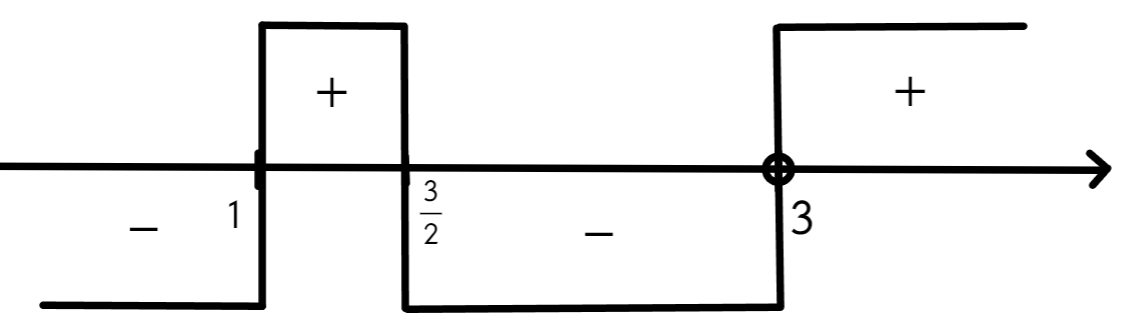
\includegraphics[scale=0.35]{ner9-75.png}}
\end{figure}\\
